\chapter{analysis}

\section{Star Tree}
	
	To do : Material on star tree, star tree analysis gives you 1 cert savings, Following tolopogies are not exactly star  

	Analysis is true for any n bit forest size.

	\textbf{Maximum savings}, with n(=4) bit forest, fanout(=2), savings of n(=4) certificates:

	\begin{multicols}{2}

		\begin{tabular}{ l | l l c r }
		  1 & 1 & 1 & 1 & 0 \\
		  \hline
		  0 & 1 & 1 & 1 & 1 \\
		  0 & 1 & 1 & 1 & 1 \\
		  0 & 0 & 0 & 0 & 1 \\
		  \hline	
		  A & C & C & C & C\\
		\end{tabular}
	\columnbreak{|}
		\begin{tabular}{ l | l l c r }
		  1 & 1 & 1 & 1 & 0 \\
		  \hline
		  0 & 1 & 1 & 1 & 1 \\
		  0 & 1 & 1 & 1 & 1 \\
		  0 & 0 & 0 & 0 & 1 \\
		  \hline	
		  A & A & A & A & A\\
		\end{tabular}
	\end{multicols}

	\textbf{No savings}, with n(=4) bit forest with alternate bit positions, fanout(=2, 3, 5) :

	\begin{multicols}{3}

		\begin{tabular}{ l |l l c r }
		  
		  1 & 0 & 1 & 0 & 0 \\
		  \hline
		  0 & 1 & 0 & 1 & 0 \\
		  0 & 1 & 0 & 1 & 0 \\
		  0 & 0 & 0 & 0 & 1 \\
		  \hline	
		  A & 0 & A & 0 & A \\
		
		\end{tabular}
		\columnbreak{|}
		\begin{tabular}{ l |l l c r }
		  
		  1 & 0 & 1 & 0 & 0 \\
		  \hline
		  0 & 1 & 0 & 1 & 0 \\
		  0 & 1 & 0 & 1 & 0 \\
		  0 & 1 & 0 & 1 & 0 \\
		  0 & 0 & 0 & 0 & 1 \\
		  \hline	
		  A & C & A & C & A \\
		
		\end{tabular}
		\columnbreak{|}
		\begin{tabular}{ l l |l l c r }
		  
		  0 & 1 & 0 & 0 & 0 & 0 \\
		  0 & 1 & 0 & 1 & 0 & 0 \\
		  1 & 1 & 1 & 1 & 0 & 0 \\
		  \hline
		  0 & 0 & 1 & 0 & 1 & 0 \\
		  0 & 0 & 1 & 0 & 1 & 0 \\
		  0 & 0 & 1 & 0 & 1 & 0 \\
		  0 & 0 & 1 & 0 & 1 & 0 \\
		  0 & 0 & 1 & 0 & 1 & 0 \\
		  0 & 0 & 0 & 0 & 0 & 1 \\
		  \hline	
		  A & A & 0 & 0 & C & A \\
		
		\end{tabular}

	\end{multicols}

	\newpage

	 \textbf{Savings of n - 1 certificates}, with n(=4) bit forest, fanout(=3) :

	\begin{multicols}{2}

		\begin{tabular}{ l l |l l c r }
		  0 & 1 & 1 & 1 & 1 & 0 \\
		  1 & 1 & 1 & 1 & 1 & 0 \\
		  \hline
		  0 & 0 & 1 & 1 & 1 & 1 \\
		  0 & 0 & 1 & 1 & 1 & 1 \\
		  0 & 0 & 1 & 1 & 1 & 1 \\
		  0 & 0 & 0 & 0 & 0 & 1 \\
		  \hline	
		  A & 0 & C & C & C & 0 \\
		\end{tabular}
	\columnbreak{|}
		\begin{tabular}{ l l | l l c r }
		  0 & 1 & 1 & 1 & 1 & 0 \\
		  1 & 1 & 1 & 1 & 1 & 0 \\
		  \hline
		  0 & 0 & 1 & 1 & 1 & 1 \\
		  0 & 0 & 1 & 1 & 1 & 1 \\
		  0 & 0 & 1 & 1 & 1 & 1 \\
		  0 & 0 & 0 & 0 & 0 & 1 \\
		  \hline
		  A & 0 & A & A & A & 0\\

		\end{tabular}

	\end{multicols}

	\textbf{Savings of n - 1 certificates}, with n(=4) bit forest, fanout(=4) :

	\begin{multicols}{2}

		\begin{tabular}{ l l |l l c r }
		  
		  0 & 1 & 1 & 1 & 0 & 0 \\
		  0 & 1 & 1 & 1 & 1 & 0 \\
		  1 & 1 & 1 & 1 & 1 & 0 \\
		  \hline
		  0 & 0 & 1 & 1 & 1 & 1 \\
		  0 & 0 & 1 & 1 & 1 & 1 \\
		  0 & 0 & 1 & 1 & 1 & 1 \\
		  0 & 0 & 1 & 1 & 1 & 1 \\
		  0 & 0 & 0 & 0 & 0 & 1 \\
		  \hline	
		  A & A & C & C & 0 & C \\
		
		\end{tabular}
	\columnbreak{|}
		\begin{tabular}{ l l | l l c r }
		  0 & 1 & 1 & 1 & 0 & 0 \\
		  0 & 1 & 1 & 1 & 1 & 0 \\
		  1 & 1 & 1 & 1 & 1 & 0 \\
		  \hline
		  0 & 0 & 1 & 1 & 1 & 1 \\
		  0 & 0 & 1 & 1 & 1 & 1 \\
		  0 & 0 & 1 & 1 & 1 & 1 \\
		  0 & 0 & 1 & 1 & 1 & 1 \\
		  0 & 0 & 0 & 0 & 0 & 1 \\
		  \hline
		  A & A & A & A & 0 & A\\

		\end{tabular}

	\end{multicols}

\newpage

\section{Pseudo Palm Tree}
	\begin{figure}[H]
		\centering
		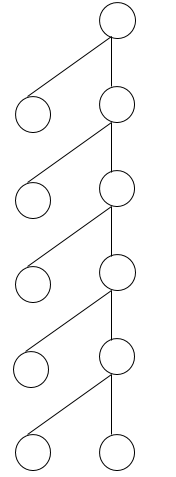
\includegraphics{images/pseudo_palm_tree}
	\end{figure}
	
	Write up:\\
	Classify nodes as aggregator vs no aggregator
	This tree has following property: \\
		Every aggregator has odd number of children\\

	\begin{multicols}{4}
		\begin{tabular}{ l | l }
			1 & 0 \\
			\hline
			0 & 1 \\
			0 & 1 \\
			0 & 1 \\
			\hline
			A & C \\
		\end{tabular}
		\columnbreak{|}
		\begin{tabular}{ l | l l }
			1 & 1 & 0 \\
			\hline
			0 & 0 & 1 \\
			0 & 0 & 1 \\
			0 & 1 & 1 \\
			\hline
			A & 0 & C \\
		\end{tabular}
		\columnbreak{|}
		\begin{tabular}{ l l l }
			0 & 1 & 0 \\
			\hline
			0 & 0 & 1 \\
			0 & 0 & 1 \\
			1 & 0 & 1 \\
			\hline
			C & A & C \\
		\end{tabular}
		\columnbreak{|}
		\begin{tabular}{ l | l l l }
			1 & 1 & 1 & 0 \\
			\hline
			0 & 0 & 0 & 1 \\
			0 & 0 & 0 & 1 \\
			0 & 1 & 1 & 1 \\
			\hline
			A & 0 & 0 & C \\
		\end{tabular}
	\end{multicols}

	\begin{multicols}{4}
		\begin{tabular}{ l | l }
			1 & 0 \\
			\hline
			0 & 1 \\
			0 & 1 \\
			0 & 1 \\
			\hline
			A & A \\
		\end{tabular}
		\columnbreak{|}
		\begin{tabular}{ l | l l }
			1 & 1 & 0 \\
			\hline
			0 & 0 & 1 \\
			0 & 0 & 1 \\
			0 & 1 & 1 \\
			\hline
			A & 0 & A \\
		\end{tabular}
		\columnbreak{|}
		\begin{tabular}{ l l l }
			0 & 1 & 0 \\
			\hline
			0 & 0 & 1 \\
			0 & 0 & 1 \\
			1 & 0 & 1 \\
			\hline
			C & A & A \\
		\end{tabular}
		\columnbreak{|}
		\begin{tabular}{ l | l l l }
			1 & 1 & 1 & 0 \\
			\hline
			0 & 0 & 0 & 1 \\
			0 & 0 & 0 & 1 \\
			0 & 1 & 1 & 1 \\
			\hline
			A & 0 & 0 & A \\
		\end{tabular}
	\end{multicols}

Meeting:

	Find cases where you can say it will be always A's.
	Analyze palm tree / pseudo palm tree 